\section{L'atmospère}
	L'atmosphère terrestre est la mince couche de gaz qui entoure la Terre.
	
	On considère que l'atmosphère à une épaisseur d'environ 120 km, hauteur à laquelle le ralentissement lié à l'atmosphère devient notable.
	\subsection{Composition}
	
	L'atmosphère est composée d'un ensemble de gaz dont la proportion est constante pratiquement dans toutes l'atmosphère. Cet ensemble de gaz est appelé \textbf{air}. Un autre gaz, la vapeur d'eau, est souvent mélangé à cet air, en proportion variable selon le temps, le lieu et l'altitude. La proportion de vapeur d'eau que peut contenir l'air va jusqu'à environ 5~\%.
	
	L'air sec est composé de :
	\begin{table}[H]
	\centering
	\begin{tabular}{|l|c|}
		\hline
		Gaz & Proportion \\
		\hline
		\hline
		Azote ($N$) & 78~\% \\
		\hline
		Oxygène ($O$) & 21~\% \\
		\hline
		Argon ($Ar$) & 0,9~\% \\
		\hline
		Autres gaz (dont Dioxyde de carbone ($CO_2$)) & 0,1~\% \\
		\hline
	\end{tabular}
	\caption{Composition de l'atmosphère terrestre}
	\end{table}
	
	
	\subsection{Structure}
	L'atmosphère a été découpée en plusieurs couches successives, dont les limites ont été fixées sur la base des discontinuités des variations de température que l'on y rencontre.
	
	\begin{figure}[H]
			\centering
			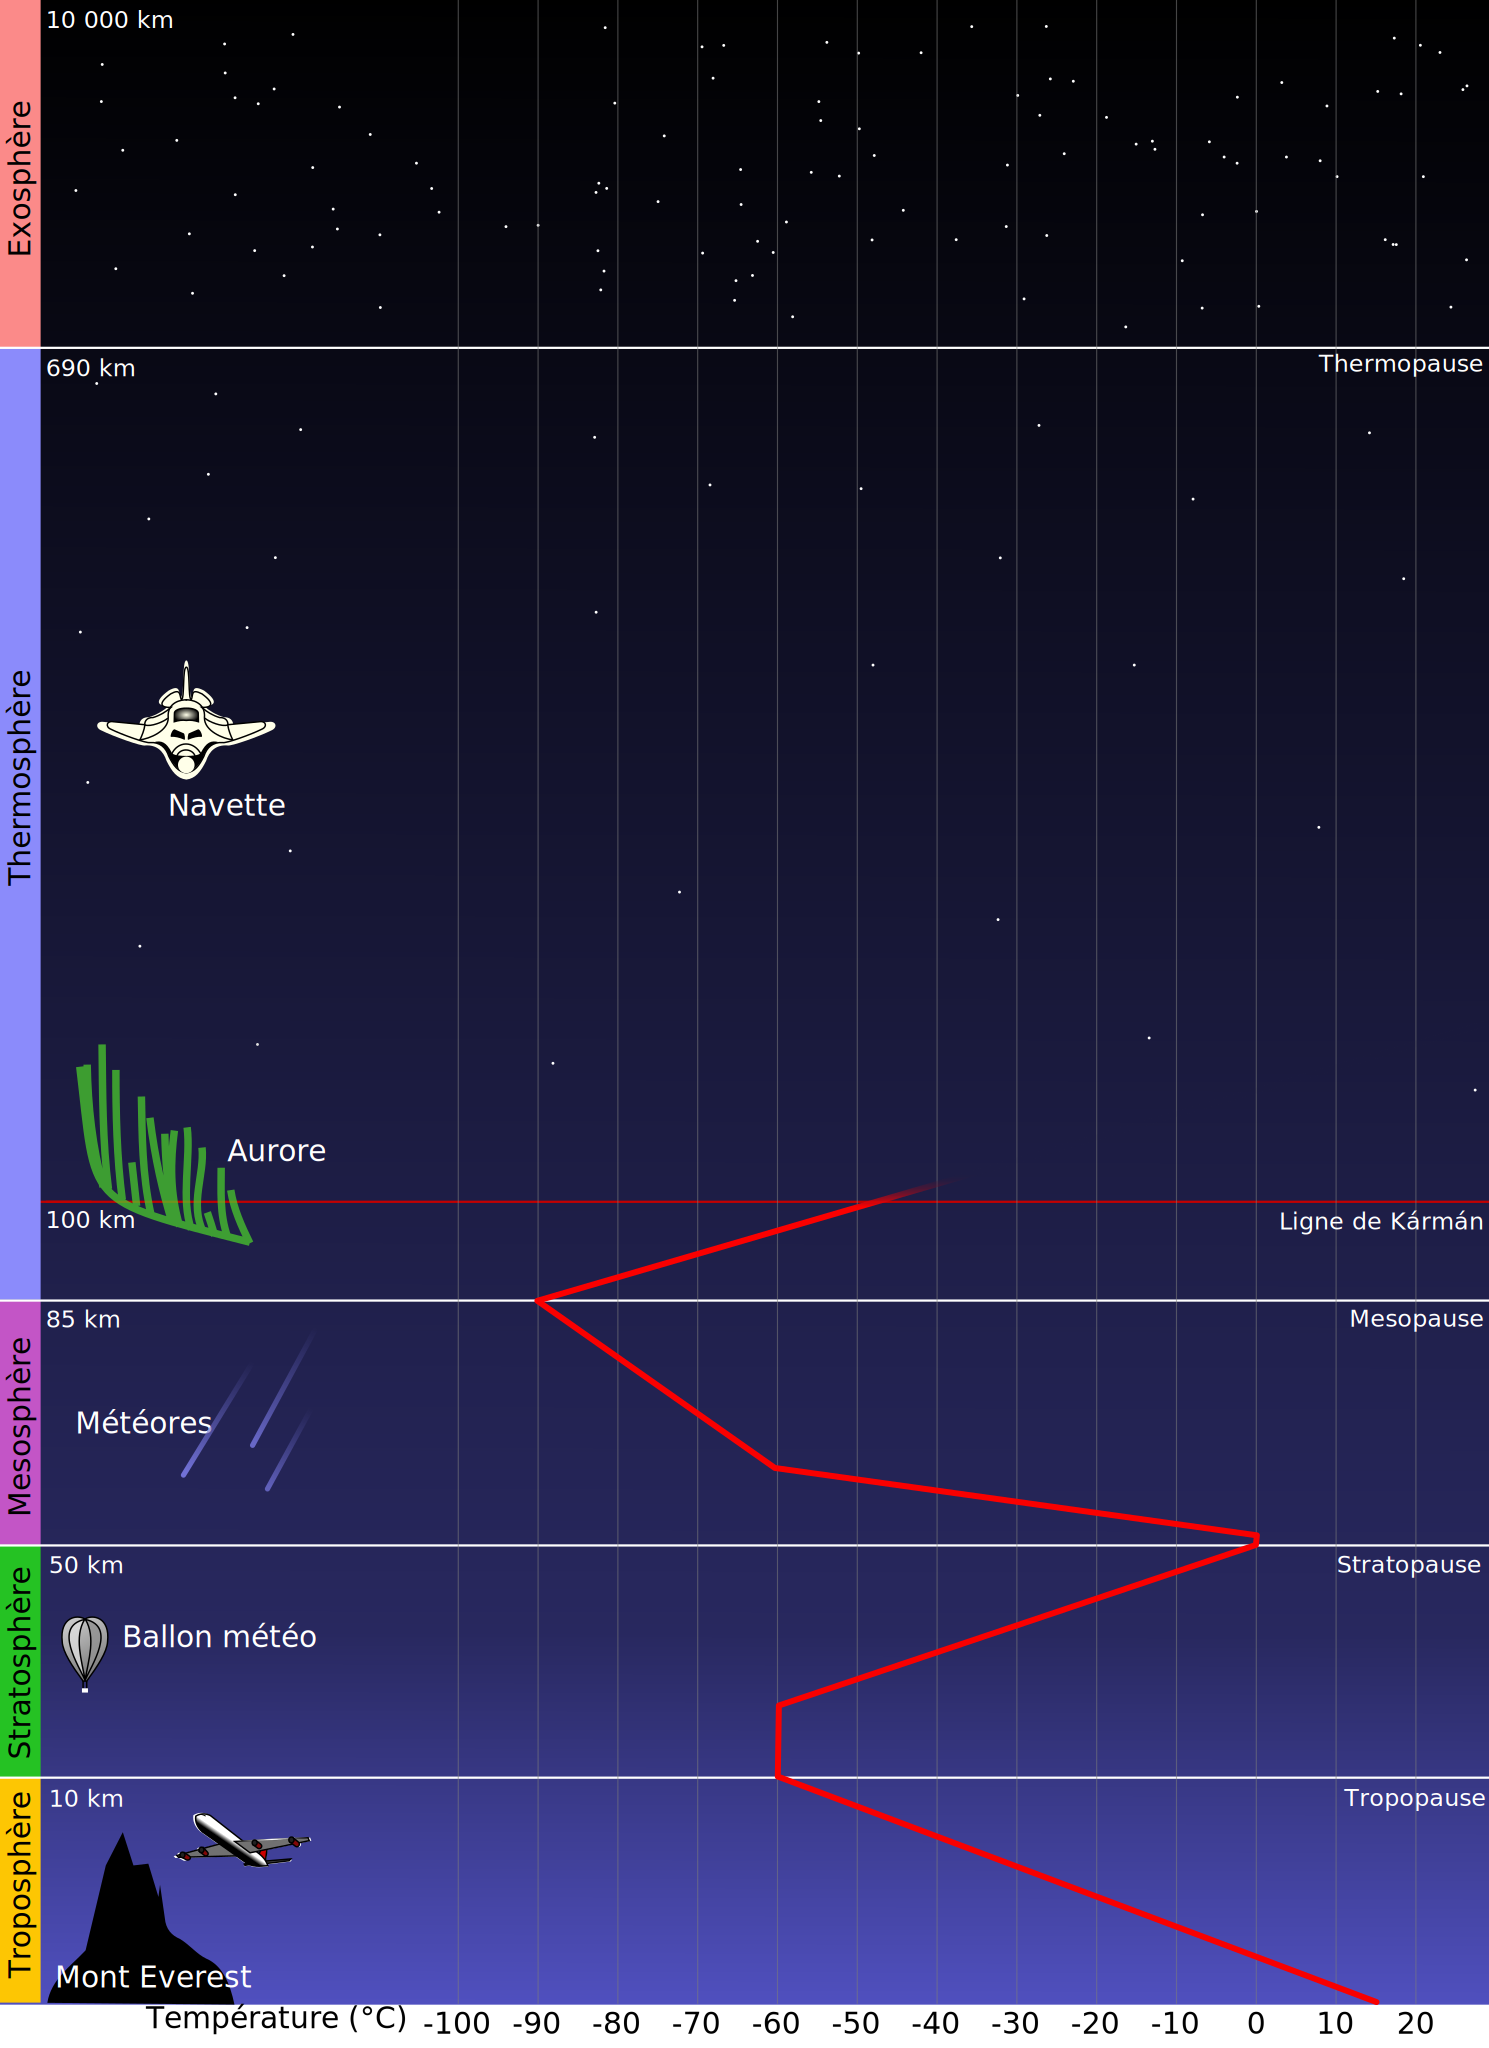
\includegraphics[width=0.8\linewidth]{03-Meteo/img/couchesAtmosphereTemperature.pdf}
			\legende{Schéma des couches de l'atmosphère, avec la courbe de température normale et le nom des limites}{img:couchesAtmosphereTemperature}
			\end{figure}	